\chapter{Experiments}\label{chapter:experiments}

In this Chapter we are going to describe the hyper-parameter search and the final structure of the best ESN on the stress prediction task. Next, we will show the settings of the ESN model, found in the previous phase, applied to the FL scenario; these phases are described in Section \ref{sec:setup}. In Section \ref{sec:results} are shown the results concerning the FL scenarios (Alg. \ref{alg:fedavg} and \ref{alg:fedcurv}) and the FL scenarios with the use of a discriminator for anomalous client detection (Alg. \ref{alg:fedavg+disc} and \ref{alg:fedcurv+disc}).


\section{Experimental Setup}\label{sec:setup}

The experiments are conducted using the Python programming language and the Machine Learning models are written using the Tensorflow framework with the Keras backend. The \textit{reservoir} of the ESN has been implemented using the Tensorflow Addons\footnote{\url{https://www.tensorflow.org/addons}} library, and specifically the \hltexttt{ESN}\footnote{\url{https://www.tensorflow.org/addons/api_docs/python/tfa/layers/ESN}} layer. The \textit{readout} of the ESN has been implemented using a simple \hltexttt{Dense}\footnote{\url{https://www.tensorflow.org/api_docs/python/tf/keras/layers/Dense}} layer with \hltexttt{Sigmoid}\footnote{\url{https://www.tensorflow.org/api_docs/python/tf/keras/activations/sigmoid}} activation function and \hltexttt{class\_weight=\{0: 12, 1: 88\}} in order to takle the problem of unbalanced labels distribution (see Table \ref{tab:data_3}). The model is compiled using the \hltexttt{Adam} optimizer\footnote{\url{https://www.tensorflow.org/api_docs/python/tf/keras/optimizers/Adam}} and \hltexttt{BinaryCrossentropy}\footnote{\url{https://www.tensorflow.org/api_docs/python/tf/keras/losses/BinaryCrossentropy}} loss function. \\

The \textit{model selection} phase is conducted using the KerasTuner\footnote{\url{https://keras.io/keras_tuner/}} library. Specifically, it is used the \hltexttt{RandomSearch}\footnote{\url{https://keras.io/api/keras_tuner/tuners/random/}} class that uses a set of \hltexttt{HyperParameters}\footnote{\url{https://keras.io/api/keras_tuner/hyperparameters/}} values to explore the search space in a random way. The dataset has been splitted in \textit{training set} containing 10 subjects, \textit{validation set} containing 4 subjects and \textit{test set} with just one subject. The search is interrupted when all the hypothesis has been exhausted. The hyper-parameter search space is shown in Table \ref{tab:grid_search}.


{\renewcommand{\arraystretch}{1.5}
\begin{table}[H]
    \centering
    \begin{tabular}{|l||c|}
        \hline
        Units & $50, 100, 200$ \\ \hline
        Leaky ($\alpha$) & $0.5, 0.8, 1.0$ \\ \hline
        Learning rate ($\eta$) & $0.001, 0.01, 0.1$ \\ \hline
        Window size & $(5\times 64), (25\times 64), (50\times 64)$ \\ \hline
        Batch size & $20, 50, 100$ \\ \hline
        Features & (pEDA, tEDA, HR, HRV), \\
        & (tEDA, pEDA), (HR, HRV), \\
        & (pEDA) \\ \hline
    \end{tabular}
    \caption{ESN hyper-parameter search space.}
    \label{tab:grid_search}
\end{table}


The best model parameters has been chosen looking at the F1 score (the harmonic mean of the precision and recall) on the \textit{validation set}. The reason why using the F1 score is that it is more suitable for task with unbalanced class distribution. In Table \ref{tab:best_model} are shown the best parameters associated with a validation F1 score of \texttt{0.9106}.

{\renewcommand{\arraystretch}{1.5}
\begin{table}[H]
    \centering
    \begin{tabular}{|c|c|c|c|c|c|c|c|}
        \hline
        Units & $\alpha$ & $\eta$ & $\rho$ & Window & Batch & Features & Epochs \\ \hline\hline
        200 & 1.0 & 0.1 & 0.99 & $25\times 64$ & 20 & pEDA & 1 \\ \hline
    \end{tabular}
    \caption{Best ESN model parameters associated with a validation F1 score of \texttt{0.9106}.}
    \label{tab:best_model}
\end{table}

A graphical representation of the  architecture of the model is shown in Fig \ref{fig:esn}.

\begin{center}
\begin{minipage}[c]{\textwidth}
    \centering
    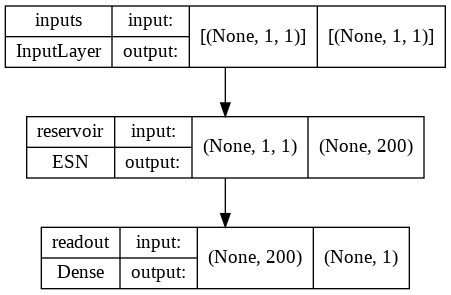
\includegraphics[width=0.7\textwidth]{contents/Chapter6/esn.png}
    \captionof{figure}{ESN model architecture.}
    \label{fig:esn}
\end{minipage}
\end{center}

In the \textit{model assessment} phase, the ESN has been re-trained on the entire \textit{design set} and having the final performances shown in Table \ref{tab:best_model_perf}.

{\renewcommand{\arraystretch}{1.5}
\begin{table}[H]
    \centering
    \begin{tabular}{|c|c|c|}
        \hline
        Accuracy (DS/TS) & AUC (DS/TS) & F1 (micro) (DS/TS) \\ \hline\hline
        $0.8986/0.9018$ & $0.8092/0.9419$ & $0.8986/0.9018$ \\ \hline
    \end{tabular}
    \caption{Best model performances on the \textit{design set} (DS) and \textit{test set} (TS).}
    \label{tab:best_model_perf}
\end{table}


After finding the best ESN model, that from now on we will call it \textit{Centralized ESN}, we need to distribute the model, using FL algorithms, in order to see how it performs. The federated learning experiments are conducted using Tensorflow-Federated\footnote{\url{https://www.tensorflow.org/federated}} framework. The experiments are divided in two phases:

\begin{enumerate}
    \item \textit{Primal phase}: the splitting of the dataset is the same as before. The \textit{training set} contains 10 subjects, \textit{validation set} contains 4 subjects and \textit{test set} with just one subject.
    
    \item \textit{Discriminative phase}: the splitting of the dataset is a little bit different. The \textit{training set} contains 10 subjects, \textit{validation set} contains 2 subjects and \textit{test set} with just one subject. The 2 subjects (that are not seen before from the \textit{Centralized ESN}) removed from the \textit{validation set} are used to train the discriminator to predict anomalous clients. The 10 clients are setup and divided into: 5 "fake" clients and 5 "real" cients. At each round 5 clients, among reals and fakes, are randomly selected. The discriminator has to discard the fake clients.
\end{enumerate}

In both phases the datasets are wrapped into the \hltexttt{ClientData}\footnote{\url{https://www.tensorflow.org/federated/api_docs/python/tff/simulation/datasets/ClientData}} class, in order to have a client for each subject. So, during the FL iterative process we have a number of 10 clients in total. Always in both phases, the parameters considered are the following:

\begin{itemize}
    \item Random number of clients to be considered at each round
    \item Injected input noise on each client, sampled from a gaussian distribution with a certain standard deviation
    \item Number of rounds (at each round the model is trained for a single epoch).
\end{itemize}

In the preliminaries results, shown in Appendix \ref{chapter:appendix}, it is noticeable that the number of clients per round, the input noise and the number of rounds are not so significant. So, the FL experiments are conducted considering the maximum number of round of \texttt{78}, the injected input noise of \texttt{0.5} and the number of clients per round of \texttt{5}. \\

In order to carry on the \textit{discriminative phase}, we have to train the discriminator. The Discriminator is a simple feedforward neural network, that accepts an input with size \texttt{201} (that corresponds to the dimension of the readout parameters), with two \hltexttt{Dense} layers, two \hltexttt{Dropout}\footnote{\url{https://www.tensorflow.org/api_docs/python/tf/keras/layers/Dropout}} layer and a \hltexttt{Dense} output layer with \hltexttt{Sigmoid} activation function. The discriminator is compiled with \hltexttt{BinaryCrossentropy} loss and \hltexttt{Adam} optimizer with a learning rate of \texttt{0.001}. The hyper-parameters have been choosen with a random search. The discriminator architecture is shown in Fig. \ref{fig:disc}.

\begin{center}
\begin{minipage}[c]{\textwidth}
    \centering
    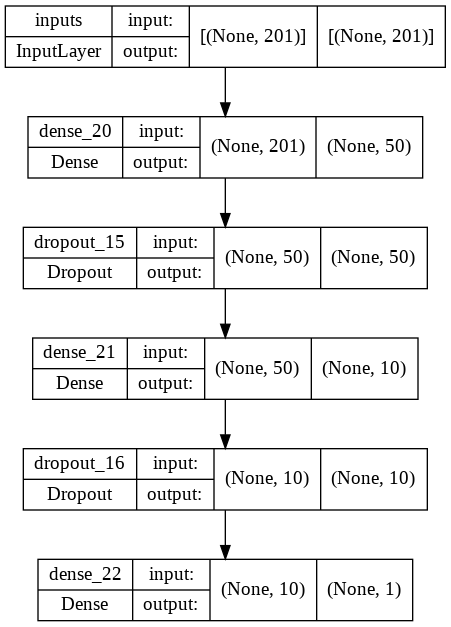
\includegraphics[width=0.7\textwidth]{contents/Chapter6/disc.png}
    \captionof{figure}{Discriminator model architecture.}
    \label{fig:disc}
\end{minipage}
\end{center}

The discriminator has to solve the problem of classifying if an ESN backpropagation gradient, during the process of stress prediction, is "real" or "fake". In order to train the discriminator we have to generate the data to give in input. 
To do so, we have instantiated two random ESN (with the same structure of Fig. \ref{fig:esn}): the \textit{Fake ESN} trained on a noisy data and \textit{Real ESN} trained on the original data. The \textit{training set} is made by the two subject extracted from the \textit{validation set} used before, instead the \textit{test set} is the same used in the previous phases. The fake data noise is generated from a gaussian distribution with standard deviation of \texttt{1.0}. The \textit{Fake ESN} reaches a test F1 score of \texttt{0.8836} and the \textit{Real ESN} reaches a test F1 score of \texttt{0.8839}. \\

The gradients collected during the training process of the \textit{Real ESN} and \textit{Fake ESN}, are divided in \textit{training set} and \textit{test set}. The \textit{training set} is fed in input to the discriminator and trained for \texttt{5} epochs, with a batch size of \texttt{64} and a validation split of 20\%. The validation binary accuracy, at the end of the process, is \texttt{0.9974}, the F1 score on the \textit{training set} is \texttt{0.9941} and the F1 score on the \textit{test set} is \texttt{0.9925}.


\section{Experimental Results}\label{sec:results}

Differently from the classical \texttt{FedAvg} (Alg. \ref{alg:fedavg}) that averages over clients weights, Tensorflow-Federated has a slightly different approach. The deltas of the clients weights after local training are sent back to the server and averaged, in order to compute a pseudo-gradient used to apply standard optimization techniques on server-side \cite{reddi2020adaptive}. \\

This implementation allow us to setup different learning rates to the server optimizer. In our experiments the server optimizer is \hltexttt{SGD}\footnote{\url{https://www.tensorflow.org/api_docs/python/tf/keras/optimizers/SGD}}, and we will use the following learning rates: \texttt{1.0}, \texttt{0.1}, \texttt{0.01}, \texttt{0.001}. The server with \hltexttt{SGD} with a learning rate of \texttt{1.0} corresponds to the classical \texttt{FedAvg} algorithm. In Figures \ref{fig:results_fl_1}, \ref{fig:results_fl_01}, \ref{fig:results_fl_001} and \ref{fig:results_fl_0001} are shown the results of the \textit{primal phase} considering \texttt{FedAvg} and \texttt{FedCurv} with different server learning rate, with clients reservoir different from the server and equal to the server; Are also considered the algorithms applied to the noisy inputs.


\begin{center}
\begin{minipage}[c]{\textwidth}
    \centering
    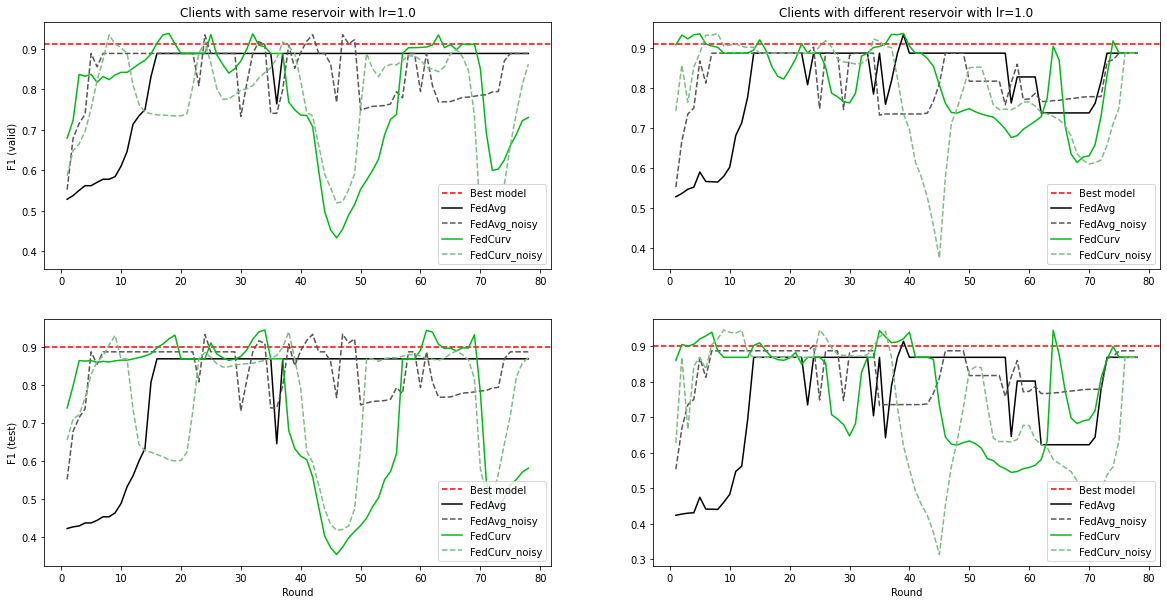
\includegraphics[width=1.0\textwidth]{contents/Chapter6/results_fl_1.png}
    \captionof{figure}{Results of the \textit{primal phase} of Federated Learning with a learning rate of \texttt{1.0}. In the left column the results with clients with the same reservoir. In the right column the results with clients with different reservoir. In the $1^{st}$ row the scores on the validation set. In the $2^{nd}$ row the scores on the test set.}
    \label{fig:results_fl_1}
\end{minipage}
\end{center}

\begin{center}
\begin{minipage}[c]{\textwidth}
    \centering
    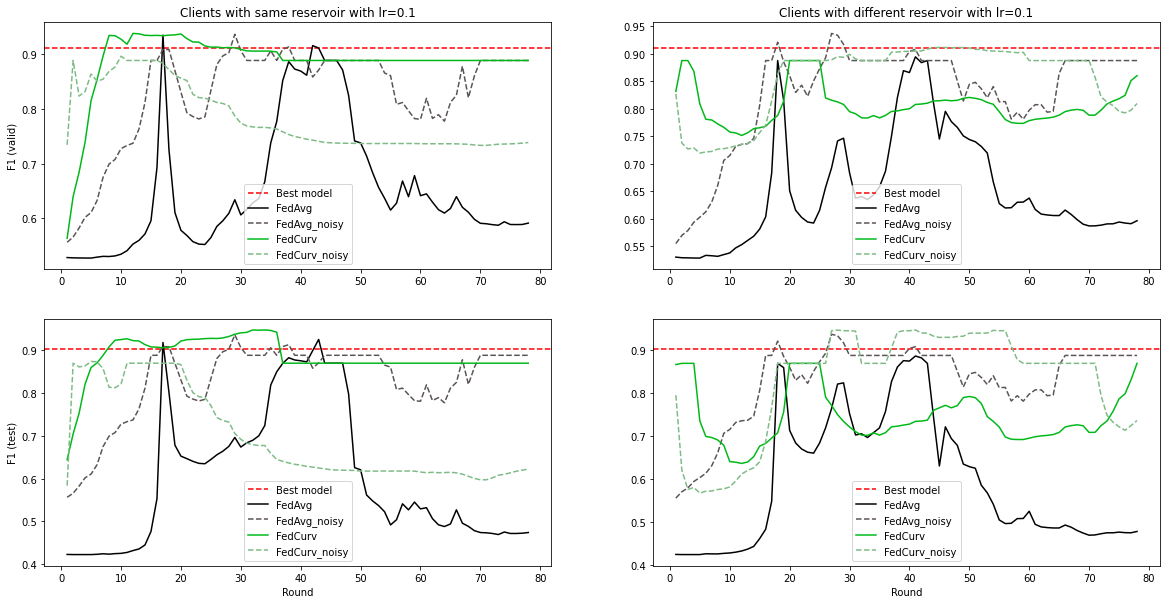
\includegraphics[width=1.0\textwidth]{contents/Chapter6/results_fl_01.png}
    \captionof{figure}{Results of the \textit{primal phase} of Federated Learning with a learning rate of \texttt{0.1}. In the left column the results with clients with the same reservoir. In the right column the results with clients with different reservoir. In the $1^{st}$ row the scores on the validation set. In the $2^{nd}$ row the scores on the test set.\\}
    \label{fig:results_fl_01}
\end{minipage}
\end{center}

\begin{center}
\begin{minipage}[c]{\textwidth}
    \centering
    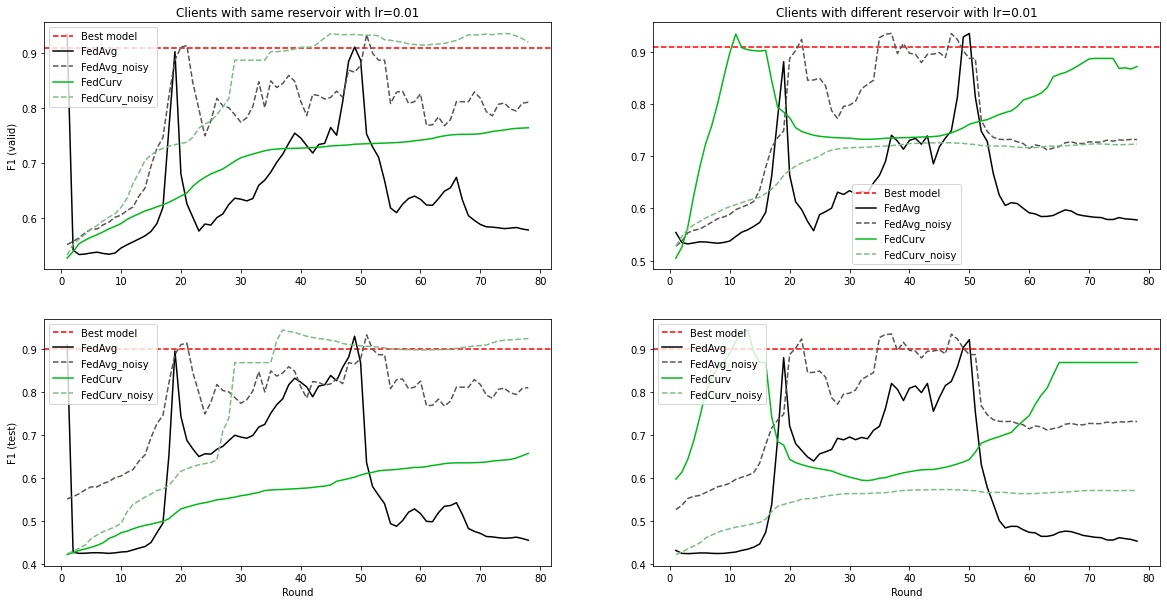
\includegraphics[width=1.0\textwidth]{contents/Chapter6/results_fl_001.png}
    \captionof{figure}{Results of the \textit{primal phase} of Federated Learning with a learning rate of \texttt{0.01}. In the left column the results with clients with the same reservoir. In the right column the results with clients with different reservoir. In the $1^{st}$ row the scores on the validation set. In the $2^{nd}$ row the scores on the test set.}
    \label{fig:results_fl_001}
\end{minipage}
\end{center}

\begin{center}
\begin{minipage}[c]{\textwidth}
    \centering
    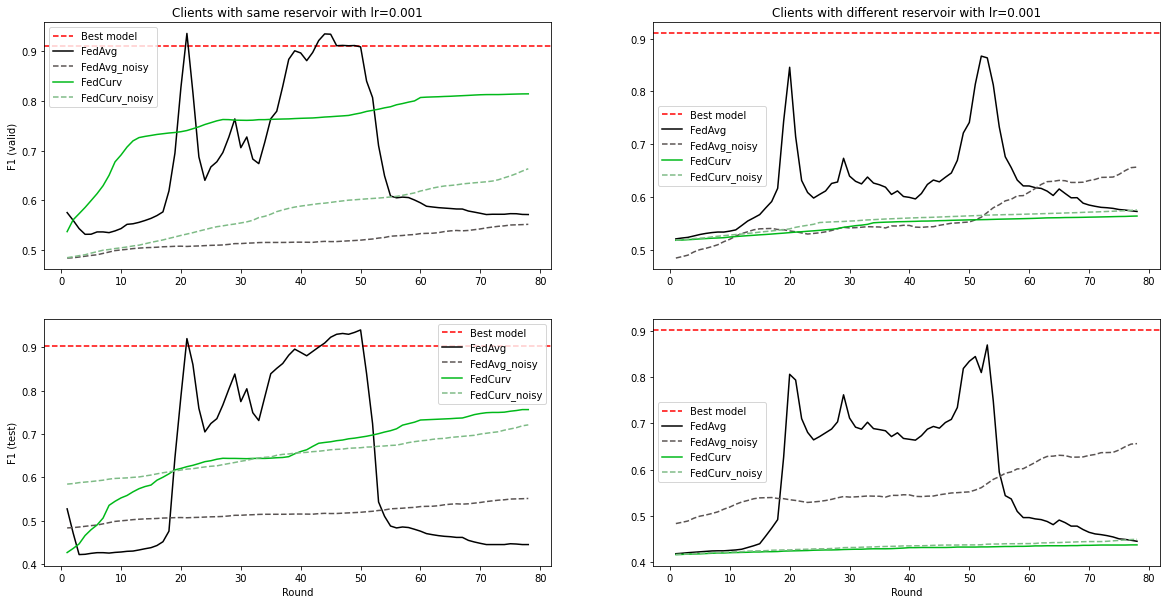
\includegraphics[width=1.0\textwidth]{contents/Chapter6/results_fl_0001.png}
    \captionof{figure}{Results of the \textit{primal phase} of Federated Learning with a learning rate of \texttt{0.001}. In the left column the results with clients with the same reservoir. In the right column the results with clients with different reservoir. In the $1^{st}$ row the scores on the validation set. In the $2^{nd}$ row the scores on the test set.\\}
    \label{fig:results_fl_0001}
\end{minipage}
\end{center}

The plots in Figures \ref{fig:results_fl_01}, \ref{fig:results_fl_001} and \ref{fig:results_fl_0001} highlights the problem of \textit{catastrofic forgetting} in \texttt{FedAvg}  with learning rates different from \texttt{1.0} and \texttt{FedCurv} alleviates this problem having more growing monotone curves. In the case of learning rate of \texttt{1.0} of Fig. \ref{fig:results_fl_1}, the algorithms have similar behaviours. \\

In Fig. \ref{fig:results_fl_comp} is shown a comparison among the best models at the last round with and without the same reservoir. We can see that \texttt{FedAvg} and \texttt{FedCurv} are similar in both cases, but \texttt{FedCurv} is able to overcome the centralized model more times than \texttt{FedAvg}. In the case of different reservoirs, we can see an unstable behaviour with respect to the case of clients with the same reservoir.

\begin{center}
\begin{minipage}[c]{\textwidth}
    \centering
    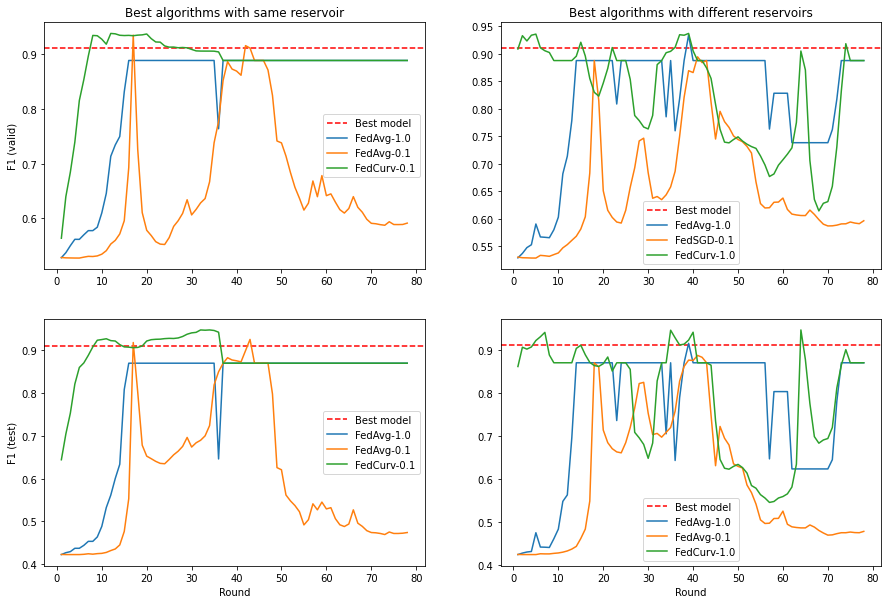
\includegraphics[width=0.8\textwidth]{contents/Chapter6/results_fl_comp.png}
    \captionof{figure}{Comparison of the best results of the \textit{primal phase} of Federated Learning. $1^{st}$ row with the scores on validation set, $2^{nd}$ row on test set. Left column with clients with the same reservoir. Right column with clients with different reservoir.\\}
    \label{fig:results_fl_comp}
\end{minipage}
\end{center}

In Figures \ref{fig:results_fl_disc_1}, \ref{fig:results_fl_disc_01}, \ref{fig:results_fl_disc_001} and \ref{fig:results_fl_disc_0001} are shown the results of the \textit{discriminative phase}, in which at each round if a client is marked as "not valid", the server uses the previous client weight and not the newest.

\begin{center}
\begin{minipage}[c]{\textwidth}
    \centering
    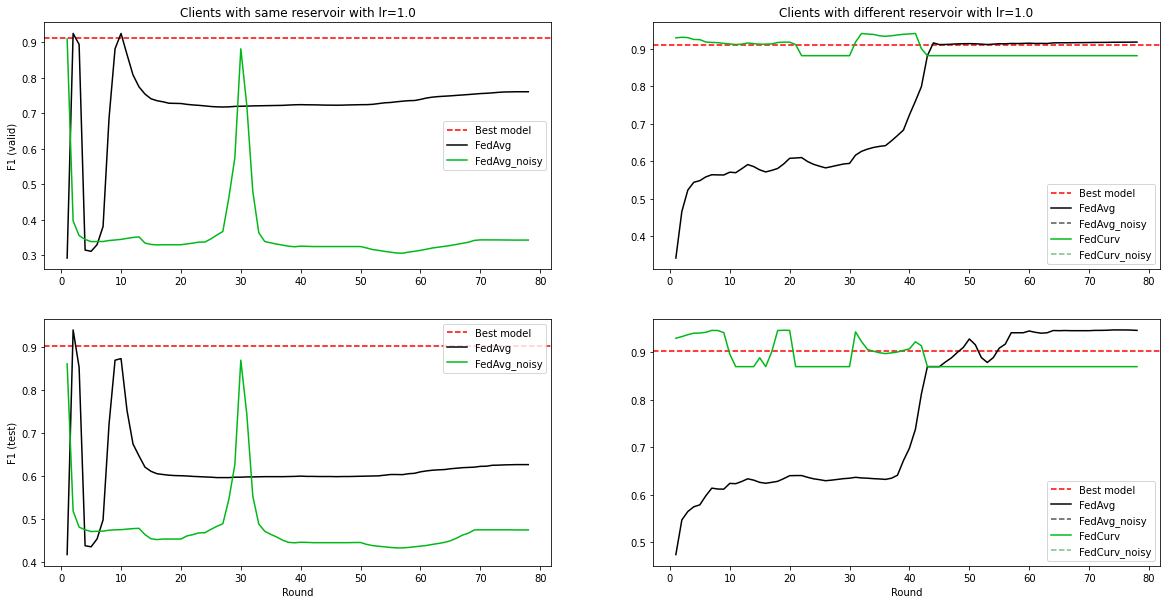
\includegraphics[width=0.8\textwidth]{contents/Chapter6/results_fl_disc_1.png}
    \captionof{figure}{Results of the \textit{discriminative phase} of Federated Learning with a learning rate of \texttt{1.0}. In the left column the results with clients with the same reservoir. In the right column the results with clients with different reservoir. In the $1^{st}$ row the scores on the validation set. In the $2^{nd}$ row the scores on the test set.\\}
    \label{fig:results_fl_disc_1}
\end{minipage}
\end{center}

\begin{center}
\begin{minipage}[c]{\textwidth}
    \centering
    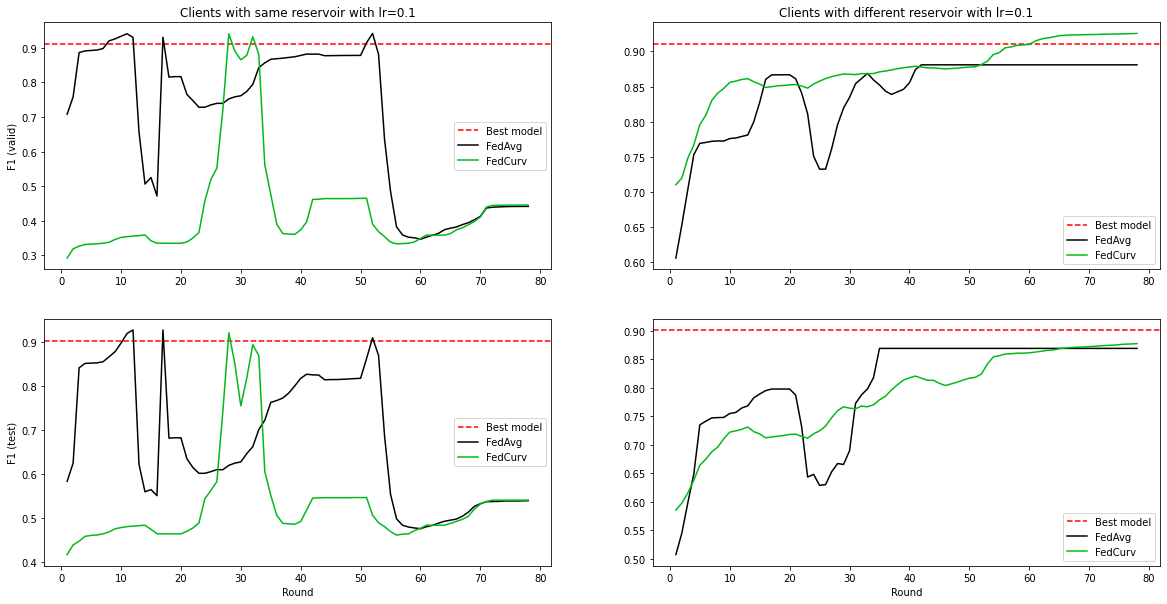
\includegraphics[width=0.8\textwidth]{contents/Chapter6/results_fl_disc_01.png}
    \captionof{figure}{Results of the \textit{discriminative phase} of Federated Learning with a learning rate of \texttt{0.1}. In the left column the results with clients with the same reservoir. In the right column the results with clients with different reservoir. In the $1^{st}$ row the scores on the validation set. In the $2^{nd}$ row the scores on the test set.\\}
    \label{fig:results_fl_disc_01}
\end{minipage}
\end{center}

\begin{center}
\begin{minipage}[c]{\textwidth}
    \centering
    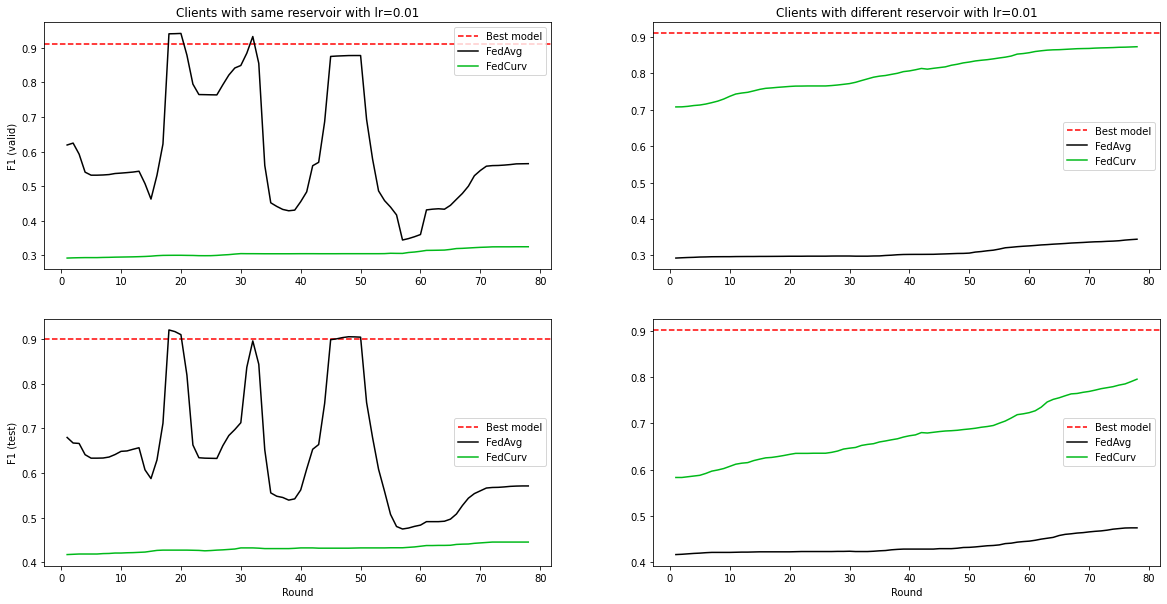
\includegraphics[width=0.8\textwidth]{contents/Chapter6/results_fl_disc_001.png}
    \captionof{figure}{Results of the \textit{discriminative phase} of Federated Learning with a learning rate of \texttt{0.01}. In the left column the results with clients with the same reservoir. In the right column the results with clients with different reservoir. In the $1^{st}$ row the scores on the validation set. In the $2^{nd}$ row the scores on the test set.\\}
    \label{fig:results_fl_disc_001}
\end{minipage}
\end{center}

\begin{center}
\begin{minipage}[c]{\textwidth}
    \centering
    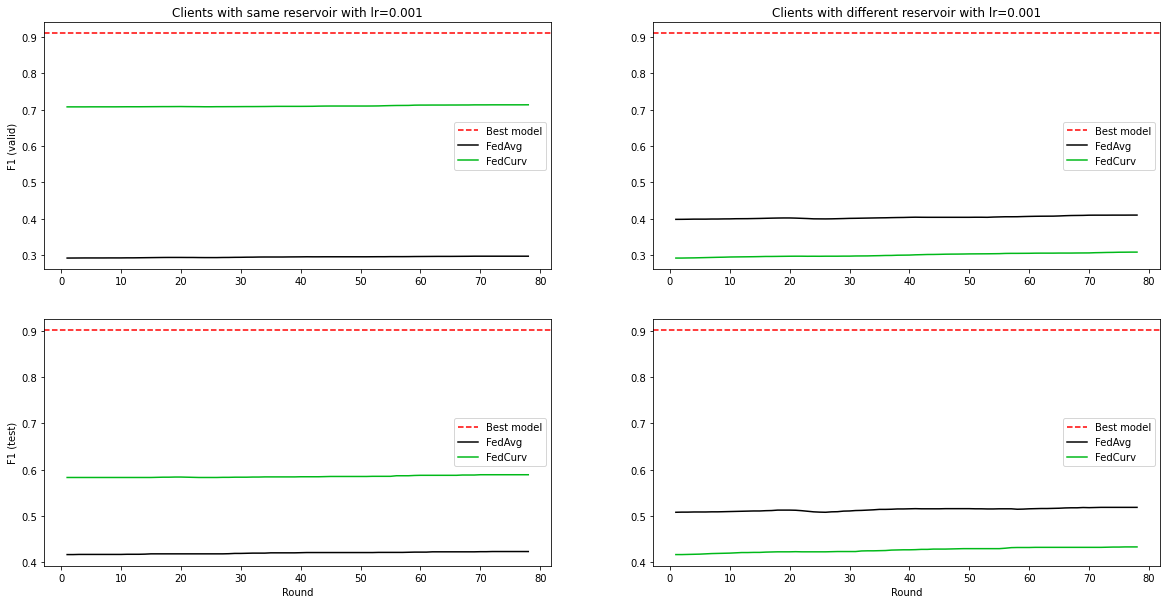
\includegraphics[width=0.8\textwidth]{contents/Chapter6/results_fl_disc_0001.png}
    \captionof{figure}{Results of the \textit{discriminative phase} of Federated Learning with a learning rate of \texttt{0.001}. In the left column the results with clients with the same reservoir. In the right column the results with clients with different reservoir. In the $1^{st}$ row the scores on the validation set. In the $2^{nd}$ row the scores on the test set.\\}
    \label{fig:results_fl_disc_0001}
\end{minipage}
\end{center}


The above results shows how the discriminator affect in a positive way the FL algorithms with different reservoir. \texttt{FedCurv} is able to match, and some times outperform, the centralized model performances; catastrofic forgetting in \texttt{FedAvg} is slightly alleviated. In Fig. \ref{fig:results_fl_disc_comp} there is a comparison of the best models of the \textit{discriminative phase}, in which we can appreciate the benefits of the discriminator in the plots in which the reservoir of the clients are different.

\begin{center}
\begin{minipage}[c]{\textwidth}
    \centering
    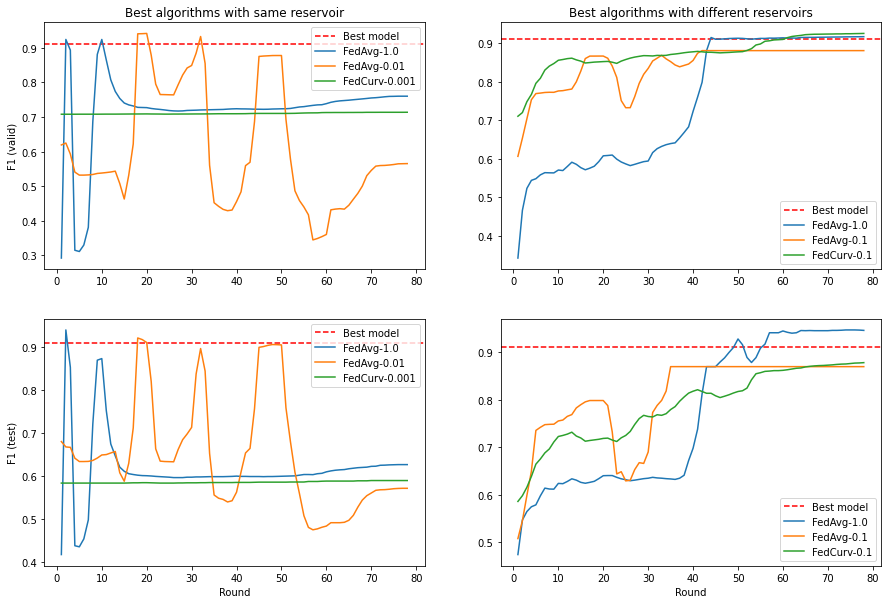
\includegraphics[width=0.8\textwidth]{contents/Chapter6/results_fl_disc_comp.png}
    \captionof{figure}{Comparison of the best results of the \textit{discriminative phase} of Federated Learning. $1^{st}$ row with the scores on validation set, $2^{nd}$ row on test set. Left column with clients with the same reservoir. Right column with clients with different reservoir.\\}
    \label{fig:results_fl_disc_comp}
\end{minipage}
\end{center}

In Table \ref{tab:final_comp} are listed the overall performances of the FL algorithm without and with the discriminator with clients having the same reservoir of the server. The SOTA ESN \cite{bacciu2021federated} solve a multi-label task, so it is not comparable with our centralized ESN that solves a binary classification task. Since, the accuracy and F1 scores of the centralized model are the same, we can compare it with the SOTA. We can notice that our centralized model overcome SOTA performances, taking in mind that the tasks are different. Looking the results of the \textit{primal phase}, no one of the FL algorithms is able to overcome the centralized model, even if the scores of the best models are close to those of the central model.

{\renewcommand{\arraystretch}{1.0}
\begin{table}[H]
    \centering
    \begin{tabular}{|l|c|c|c|c|}
        \hline
        ESN Models & Train Acc. & Test Acc. & Train F1 & Test F1 \\ \hline\hline
        
        \texttt{SOTA} (multi-label class.) & 0.8378 & 0.7792 & - & - \\ \hline
        \texttt{Central} (binary class.) & 0.8986 & 0.9018 & 0.8986 & \textbf{0.9018} \\ \hline
        \texttt{FedAvg-1.0} & - & - & 0.8878 & \textbf{0.8693} \\ \hline
        \texttt{FedAvg-0.1} & - & - & 0.5913 & 0.4741 \\ \hline
        \texttt{FedAvg-0.01} & - & - & 0.5784 & 0.4560 \\ \hline
        \texttt{FedAvg-0.001} & - & - & 0.5711 & 0.4451 \\ \hline
        \texttt{FedCurv-1.0} & - & - & 0.7299 & 0.5813 \\ \hline
        \texttt{FedCurv-0.1} & - & - & 0.8878 & \textbf{0.8693} \\ \hline
        \texttt{FedCurv-0.01} & - & - & 0.7646 & 0.6580 \\ \hline
        \texttt{FedCurv-0.001} & - & - & 0.8140 & 0.7562 \\ \hline
        \texttt{FedAvg-1.0+Disc} & - & - & 0.7601 & 0.6262 \\ \hline
        \texttt{FedAvg-0.1+Disc} & - & - & 0.4415 & 0.5392 \\ \hline
        \texttt{FedAvg-0.01+Disc} & - & - & 0.5652 & 0.5710 \\ \hline
        \texttt{FedAvg-0.001+Disc} & - & - & 0.2972 & 0.4233 \\ \hline
        \texttt{FedCurv-1.0+Disc} & - & - & 0.3427 & 0.4741 \\ \hline
        \texttt{FedCurv-0.1+Disc} & - & - & 0.4456 & 0.5405 \\ \hline
        \texttt{FedCurv-0.01+Disc} & - & - & 0.3251 & 0.4451 \\ \hline
        \texttt{FedCurv-0.001+Disc} & - & - & 0.7136 & 0.5891 \\ \hline
    \end{tabular}
    \caption{Overall comparison of the best models with different FL algorithms. The reservoirs of the clients in all the FL algorithms are \underline{equal} to the server.}
    \label{tab:final_comp}
\end{table}

In Table \ref{tab:final_comp_diff} are listed the overall performances of the FL algorithm with and without the discriminator with clients having different reservoir from the server. We can notice that classical \texttt{FedAvg} algorithm in combination with the discriminator is able to exceed the central model performances.

{\renewcommand{\arraystretch}{1.0}
\begin{table}[H]
    \centering
    \begin{tabular}{|l|c|c|c|c|}
        \hline
        ESN Models & Train Acc. & Test Acc. & Train F1 & Test F1 \\ \hline\hline
        
        \texttt{SOTA} (multi-label class.) & 0.8378 & 0.7792 & - & - \\ \hline
        \texttt{Central} (binary class.) & 0.8986 & 0.9018 & 0.8986 & \textbf{0.9018} \\ \hline
        \texttt{FedAvg-1.0} & - & - & 0.8878 & 0.8693 \\ \hline
        \texttt{FedAvg-0.1} & - & - & 0.5965 & 0.4772 \\ \hline
        \texttt{FedAvg-0.01} & - & - & 0.5779 & 0.4538 \\ \hline
        \texttt{FedAvg-0.001} & - & - & 0.5723 & 0.4457 \\ \hline
        \texttt{FedCurv-1.0} & - & - & 0.8878 & 0.8693 \\ \hline
        \texttt{FedCurv-0.1} & - & - & 0.8603 & 0.8693 \\ \hline
        \texttt{FedCurv-0.01} & - & - & 0.8722 & 0.8693 \\ \hline
        \texttt{FedCurv-0.001} & - & - & 0.5636 & 0.4379 \\ \hline
        \texttt{FedAvg-1.0+Disc} & - & - & 0.9172 & \textbf{0.9457} \\ \hline
        \texttt{FedAvg-0.1+Disc} & - & - & 0.8810 & 0.8693 \\ \hline
        \texttt{FedAvg-0.01+Disc} & - & - & 0.3440 & 0.4744 \\ \hline
        \texttt{FedAvg-0.001+Disc} & - & - & 0.4103 & 0.5187 \\ \hline
        \texttt{FedCurv-1.0+Disc} & - & - & 0.8810 & 0.8693 \\ \hline
        \texttt{FedCurv-0.1+Disc} & - & - & 0.9257 & \textbf{0.8778} \\ \hline
        \texttt{FedCurv-0.01+Disc} & - & - & 0.8733 & 0.7955 \\ \hline
        \texttt{FedCurv-0.001+Disc} & - & - & 0.3084 & 0.4332 \\ \hline
    \end{tabular}
    \caption{Overall comparison of the best models with different FL algorithms. The reservoirs of the clients in all the FL algorithms are \underline{different} from the server.}
    \label{tab:final_comp_diff}
\end{table}

In Fig. \ref{fig:valid_found} we can see a detail of the discriminative process during rounds of \texttt{FedAvg-1.0+Disc} with different reservoir. The discriminator has a Mean Absolute Error of \texttt{1.1410}. So at each round, on average, it wrongly recognizes one client as valid.

\begin{center}
\begin{minipage}[c]{\textwidth}
    \centering
    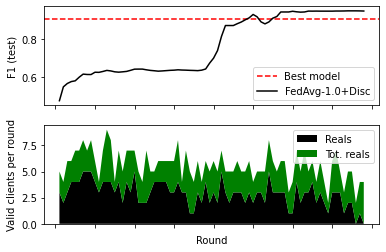
\includegraphics[width=0.9\textwidth]{contents/Chapter6/valid_found.png}
    \captionof{figure}{At the top part the \texttt{FedAvg-1.0+Disc} with different reservoir scores on test set. At the bottom part the stack plot of the \texttt{Disc} predictions of valid clients (black) vs real valid clients (green) at each round. The \texttt{Disc} predictions Mean Absolute Error is $1.1410$. \\}
    \label{fig:valid_found}
\end{minipage}
\end{center}
